%==============================================================================    
\chapter{Front-end electronics}
\label{sec:FE_electronics}
%==============================================================================    

\section{Calibration} \label{sec:calibration}
\subsection{Energy and time calibration} \label{sec:TOT_TOA_calibration}
\subsection{Threshold calibration} \label{sec:threshold}


The operating threshold DAC (Digital-to-Analog Converter) set in each
Timepix/Timepix3 readout chip can be translated into an effective
energy and used as a data point for the surrogate fit at the
crossing-point on the $x$-axis. The counting (Medipix) mode was used
for this measurement. The assembly was exposed to photons of a
characteristic energy and the threshold DAC was scanned from a level
of no counts (threshold above the signal) to a level where all the
pixels count (threshold close to the noise level) resulting in an
S-shaped curve as shown in \cref{fig:scurve_example}. At the
maximum gradient of the S-curve, the threshold DAC corresponds to the
photon energy. The derivative of the S-curve is a Gaussian as shown in
\cref{fig:deriv_example} with a mean at the maximum gradient of
the S-curve. The derivative at each point of the S-curve corresponds
to the slope of the line connecting it to its neighbour.

\begin{figure}[htbp] \centering
  \begin{subfigure}[b]{0.45\textwidth}
    \begin{tikzpicture} \node[anchor=south west,inner sep=0] (image)
      at
      (0,0){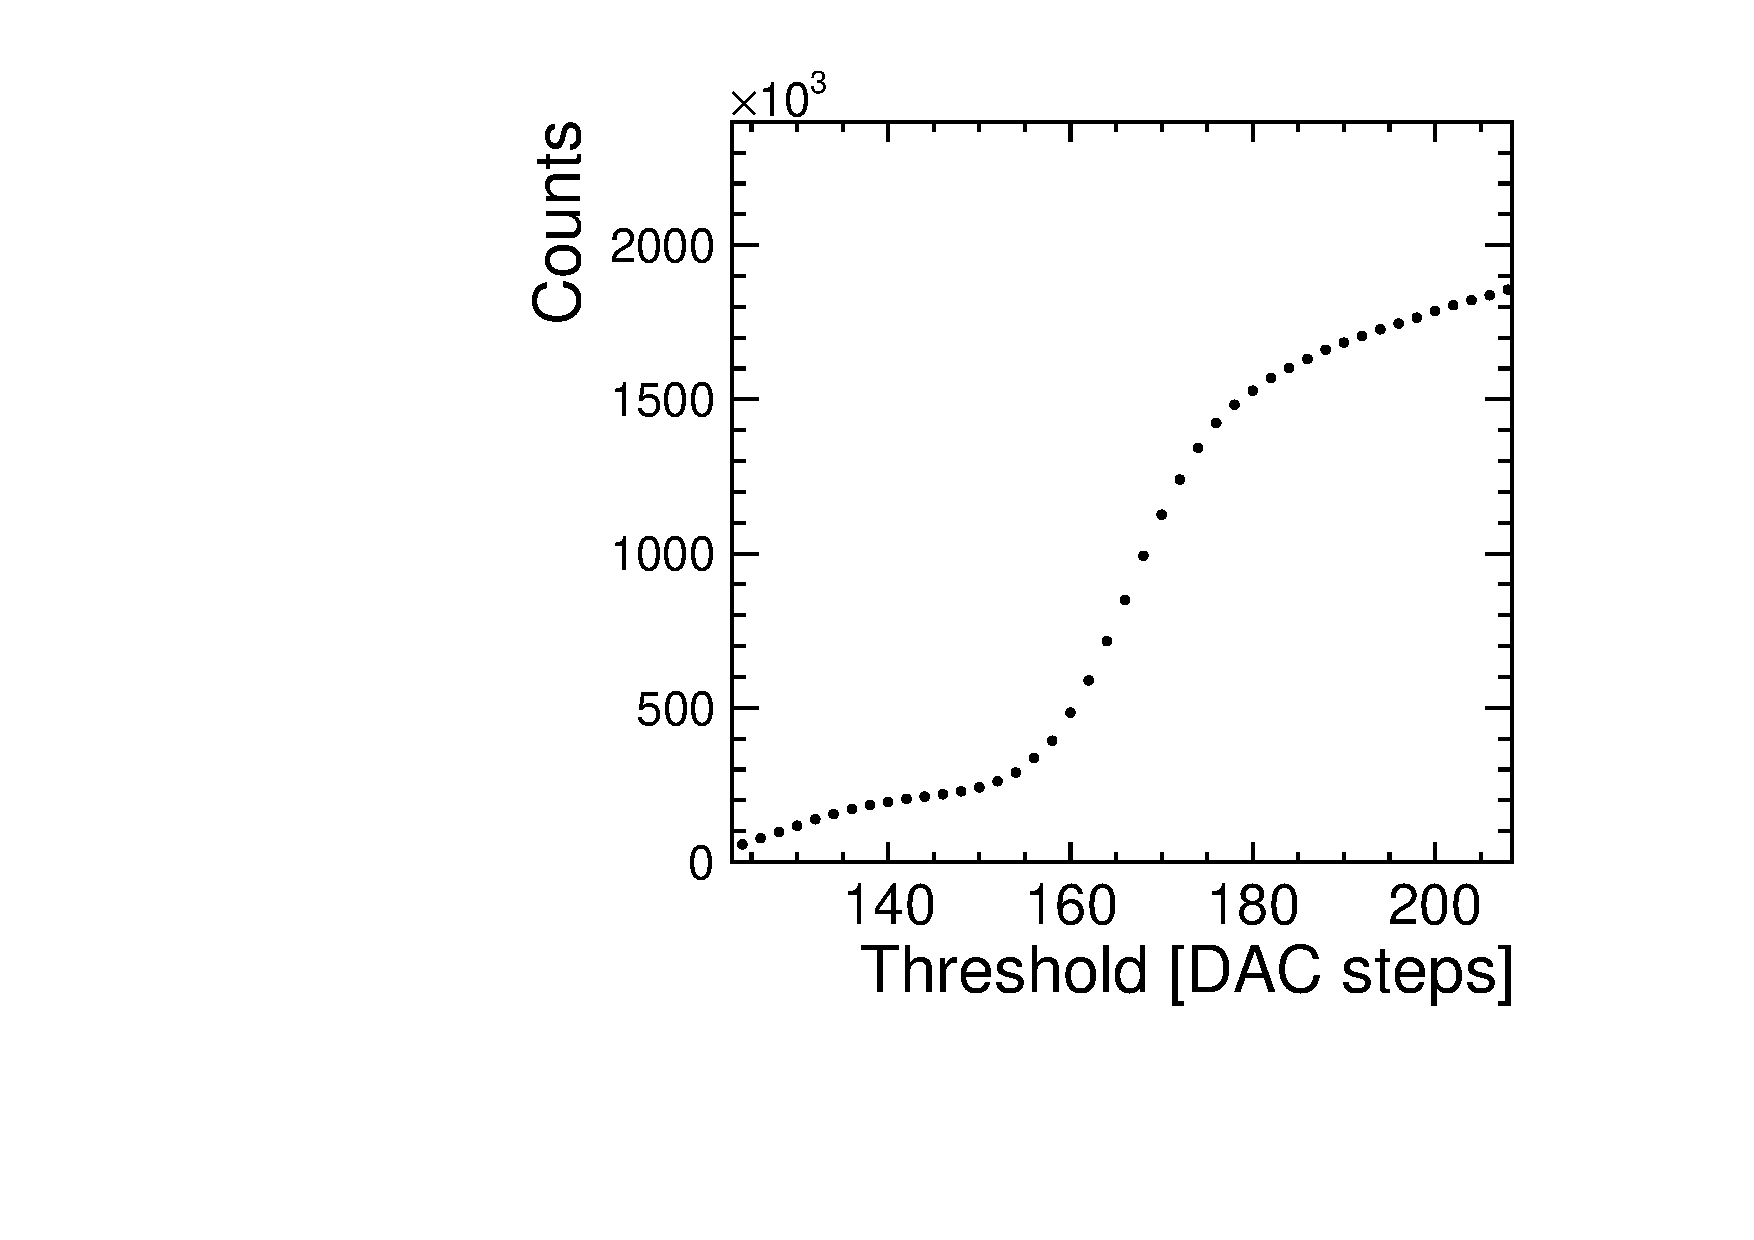
\includegraphics[width=\textwidth]{./figures/Calibration/L04-W0125_scurve_In.pdf}};
      % \draw[->,line width=.4pt, color=black](1.8, 1.4) -- (2.4, 1.4);
      \node[left, color=black] at (1.9, 1.6) {$K_{\beta}$}; %\draw[->,line
      width=.4pt, color=black](3, 2.7) -- (3.7, 2.7); \node[left,
      color=black] at (3.5, 2.7) {$K_{\alpha}$};
    \end{tikzpicture}
    \caption{Measured S-curve}
    \label{fig:scurve_example}
  \end{subfigure} \hfill
  \begin{subfigure}[b]{0.45\textwidth}
    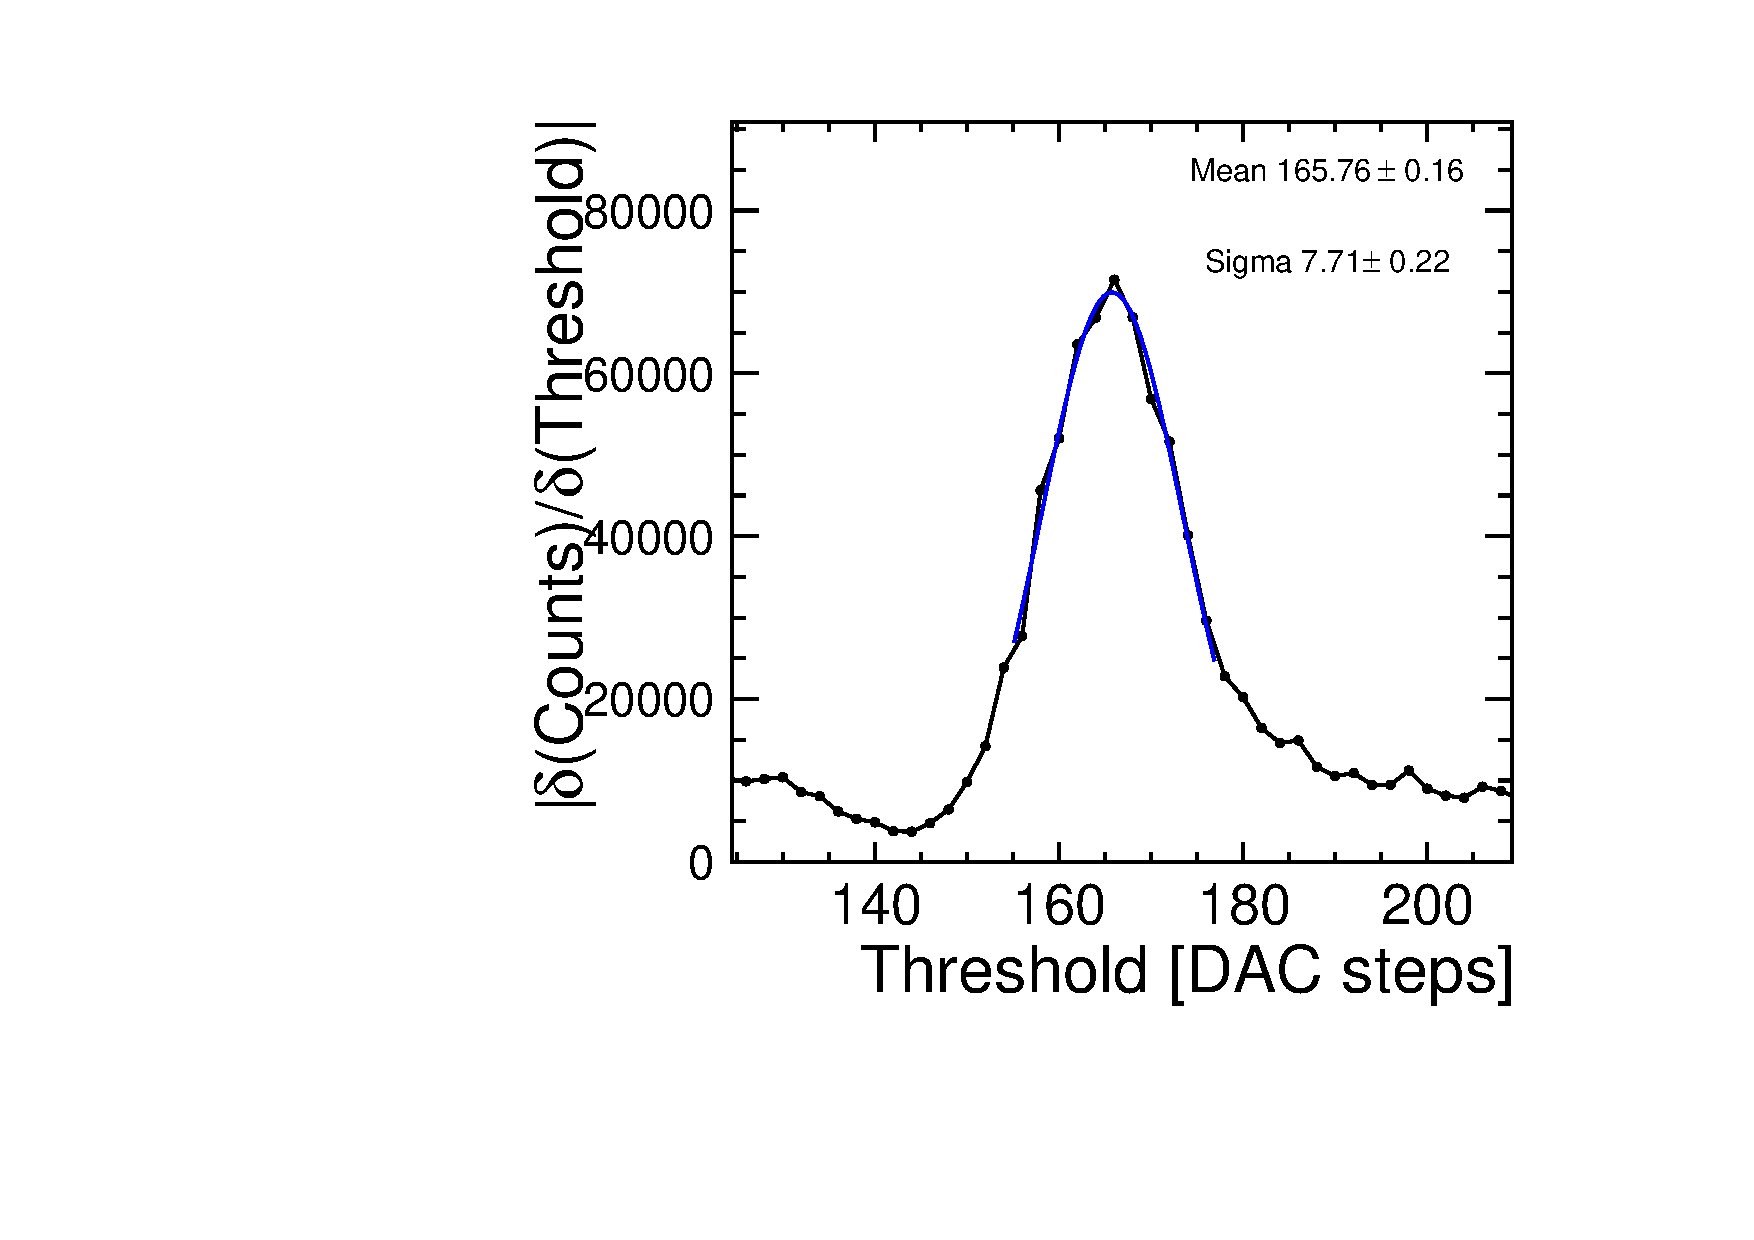
\includegraphics[width=\textwidth]{./figures/Calibration/L04-W0125_scurveDeriv_In.pdf}
    \caption{Derivative of the S-curve}
    \label{fig:deriv_example}
  \end{subfigure}
  \caption{An example of a measured S-curve (a) and its derivative
    fitted with a Gaussian function (b) for L04-W0125 (Timepix readout
    ASIC) using the Indium target. $K_{\alpha}$ corresponds to the
    strongest X-ray spectral line for the bombarded target. The smaller
    peak for $K_{\beta}$ is ignored. For Timepix assemblies. The Pixelman
    software~\cite{1748-0221-6-01-C01046} provides the \emph{DACs Scan}
    plug-in which was used to scan the threshold DAC value and save the
    hit maps in a text file. The threshold calibration was done at CERN
    using the XRF targets. This measurement was performed globally for
    each assembly. The threshold DAC is scanned with a step size of 2.}
  \label{fig:scurve_deriv_example}
\end{figure}

A linear fit was used to parametrise the relationship between the
photon energy and the threshold DAC given by the mean of the
derivative of the S-curves:
\begin{equation}
  THL_{DAC}=p \; THL_{\kev} + q \; ,
  \label{eq:THLDAC}
\end{equation}
where $THL_{DAC}$ is the threshold DAC and $THL_{\kev}$ its conversion
into an energy. \cref{fig:THLcalib_A06} shows an example of the
threshold calibration obtained for A06-W0110. Each point used for the
fit corresponds to the mean of the Gaussian fitted to the derivative
of the S-curve for each target. The error on each point corresponds to
the error on the mean of the fitted Gaussian.

\begin{figure}[htbp]
  \centering
  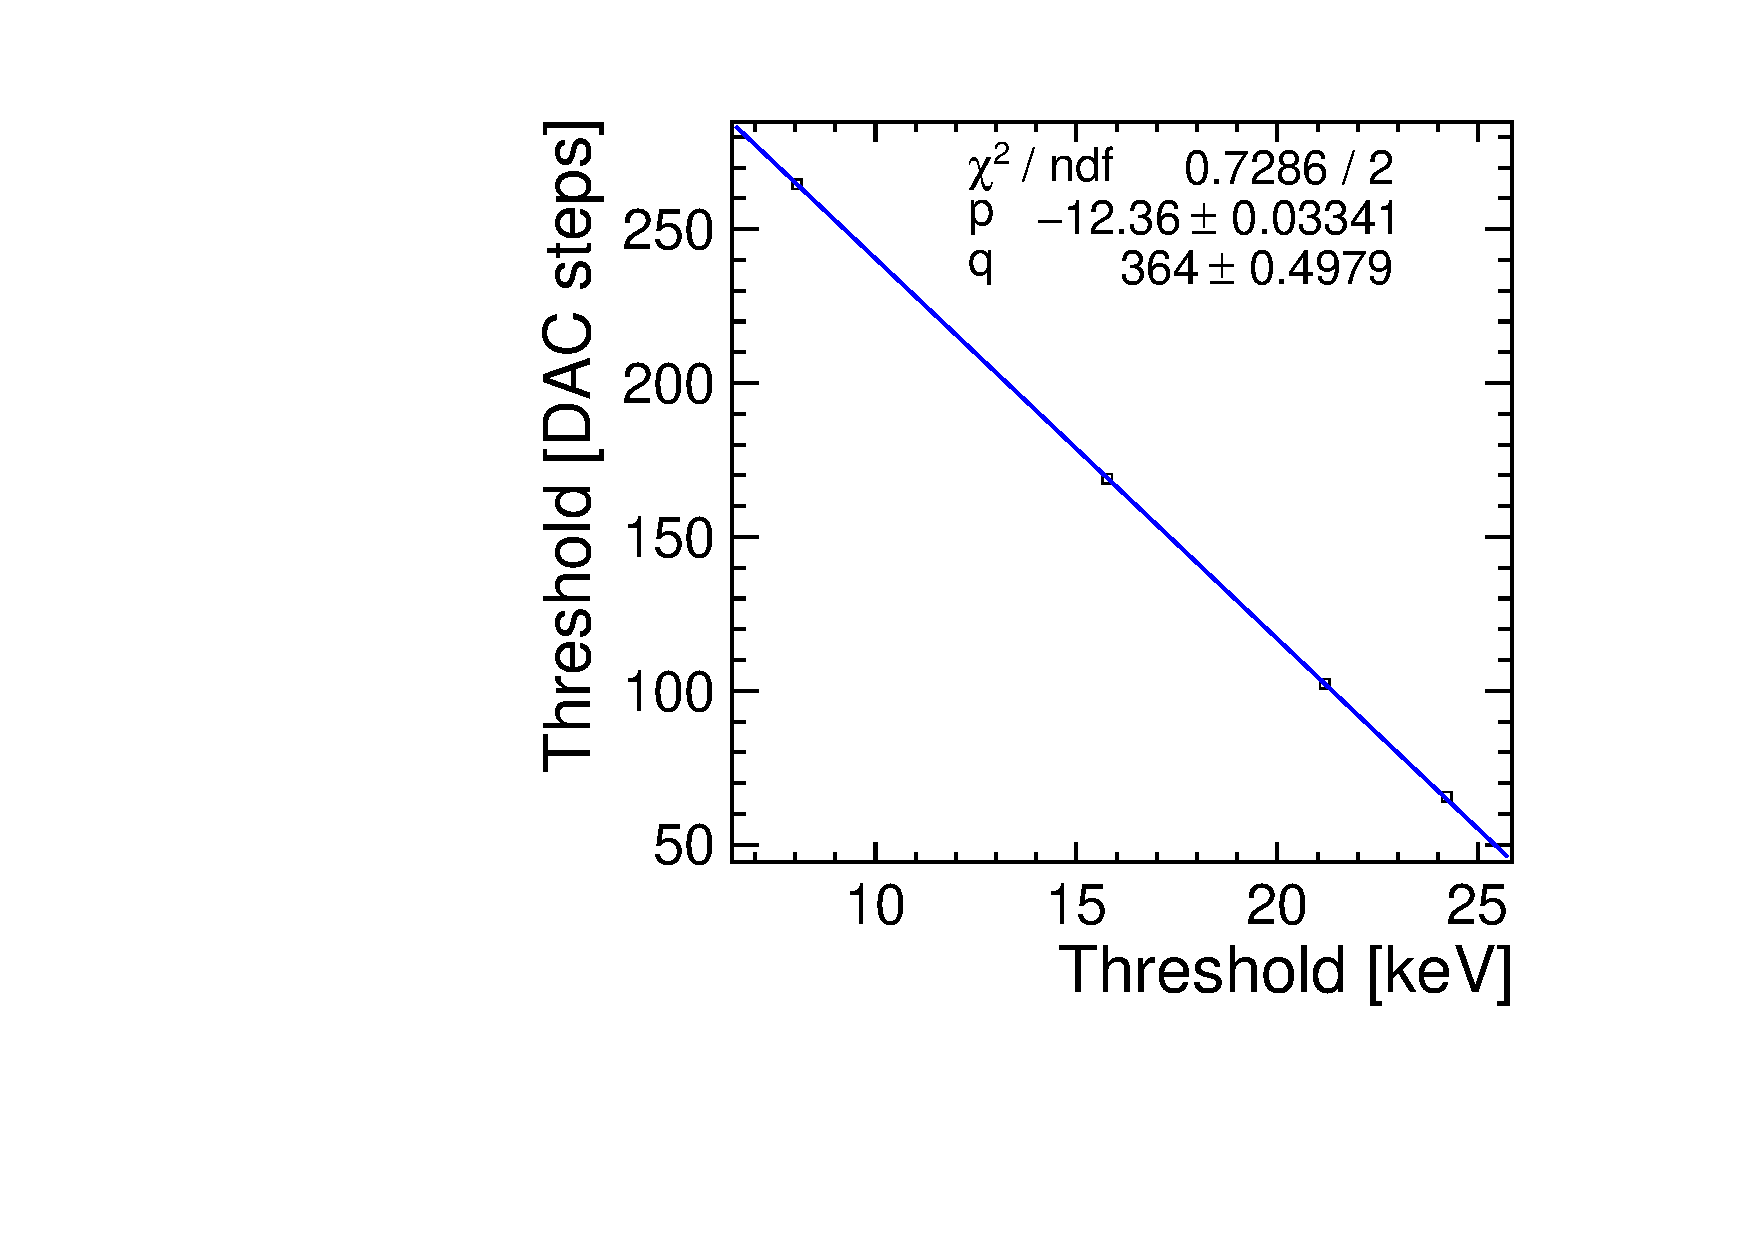
\includegraphics[width=0.5\textwidth]{./figures/Calibration/A06-W0110_THLcalibration.pdf}
  \caption{Threshold calibration for A06-W0110. Each point corresponds
    to the maximum gradient of the S-curve for each target (Cu, Zr, Pd
    and In). A linear function as described in \cref{eq:THLDAC} was
    used to fit the data points and obtain the parameters $p$ and
    $q$.}
  \label{fig:THLcalib_A06}
\end{figure}

The operating threshold DAC for each assembly was converted to an
energy by solving \cref{eq:THLDAC} for $THL_{\kev}$ with
$THL_{DAC}=THL_{DAC}^{op}$. Results are shown in \cref{tab:evalTHL}. The error on the evaluated threshold in energy
($THL_{\kev}^{op}$) is obtained by the propagation of errors for the
inverse of \ref{eq:THLDAC}:
\begin{equation}
  \sigma_{THL_{\kev}}^2(THL_{DAC})={{{(THL_{DAC}-q)^2} \over {p^4}} \sigma_{p}^2} +
        {\frac{1}{p^2} \sigma_{q}^2}+
        {2 {{THL_{DAC}-q} \over p^3} \sigma_{pq}^2} \; ,
        \label{eq:THLerror}
\end{equation}
where $p$, $q$ are given by the linear fit using \ref{eq:THLDAC} with
standard deviations $\sigma_{p}$, $\sigma_{q}$ and covariance
$\sigma_{pq}$.

\begin{table}[htbp]
  \caption{Threshold fit parameters $p$ and $q$, the operating
    threshold DAC and its conversion into energy.}
  \label{tab:evalTHL} 
  \centering
  \begin{tabular}{ c c c c c }
    \toprule
    Assembly & $p$ [DAC steps/\kev] & $q$ [DAC steps] & $THL_{DAC}^{op}$ [DAC steps] & $THL_{\kev}^{op}$ [\kev] \\
    \midrule
    A06-W0110 & $-12.36\pm0.03$ & $364.0\pm0.50$ & 326 & $3.077\pm0.033$ \\
    C04-W0110 & $-11.8\pm0.02$ & $441.6\pm0.42$ & 405 & $3.102\pm0.030$ \\
    L04-W0125 & $-11.68\pm0.02$ & $448.6\pm0.31$ & 410 & $3.303\pm0.023$ \\
    B06-W0125 & $11.58\pm0.037$ & $390.6\pm0.80$ & 435 & $3.836\pm0.057$ \\
    \bottomrule
  \end{tabular}
\end{table}

% For further verification of these results, the DAC step gain for each
% assembly was calculated to be around 24~\Pem/step (see
% \ref{tab:DACStep}), in agreement with~\cite{art:tmpx}. The width of
% the derivative of the S-curves shows the error at the front-end of the
% assembly. For all assemblies it varies between 7 to 11 DAC values
% which corresponds to 170 to 270 electrons, again in agreement
% with~\cite{art:tmpx} (the error is obtained by error propagation of
% \ref{eq:THLDAC}).



% \begin{table}[htbp]
%   \caption{Measured DAC step gain.}
%   \label{tab:DACStep}
%   \centering
%   \begin{tabular}{ c c c }
%     \toprule
%     Assembly & Threshold DAC step [\ev] & Threshold DAC step [\Pem] \\
%     \midrule
%     A06-W0110  & $81\pm0.009$ & $22.475\pm0.025$  \\
%     C04-W0110  & $85\pm0.039$ & $23.544\pm0.011$ \\
%     L04-W0125 &  $86\pm0.022$ & $23.775\pm0.006$ \\
%     B06-W0125  & $86\pm0.120$ & $23.978\pm0.033$ \\
%     \bottomrule
%   \end{tabular}
% \end{table}

% Threshold measurements were not completed for assemblies B07-W0125 and
% D09-W0126. Assembly B07-W0125 did not fully deplete due to a broken
% corner of the sensor. The derivative of the CuXRF S-curve did not form
% a peak as the photon energy was close to the noise level. Assembly
% D09-W0126 was not operating as expected for a $100\,\micron$
% sensor. Therefore the calibration of these assemblies was done without
% threshold measurements.